% Figure 2: Axis 1 - Log-Linear Regression log10(T) vs Length L
\begin{figure}[htbp]
\centering
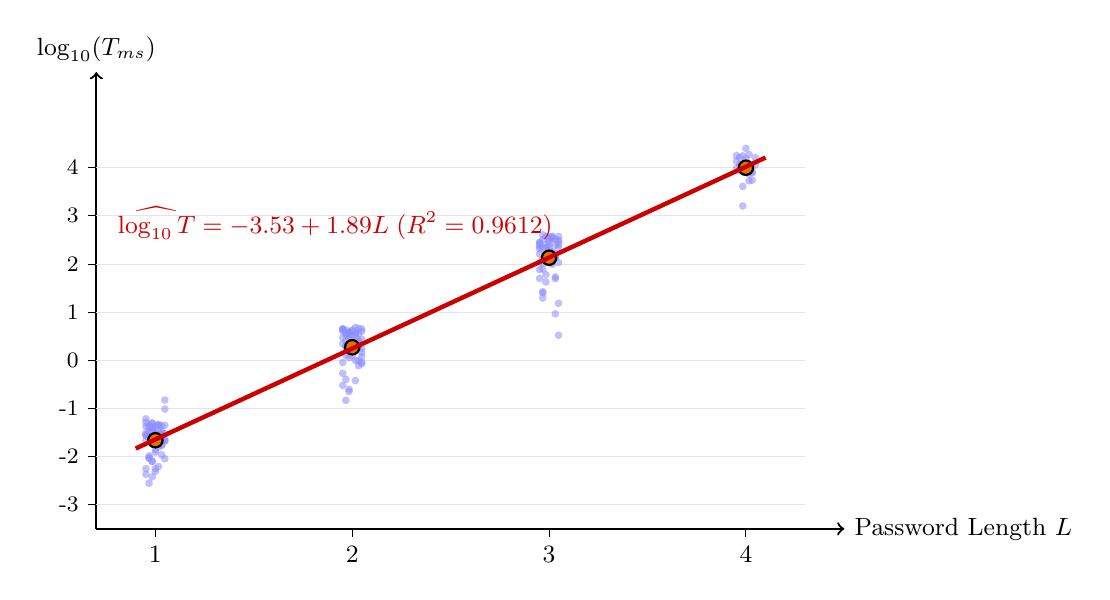
\begin{tikzpicture}[xscale=1.0, yscale=1.0]
  \draw[->, thick] (0,0) -- (9.5,0) node[right, font=\small] {Password Length $L$};
  \draw[->, thick] (0,0) -- (0,5.8) node[above, font=\small] {$\log_{10}(T_{\text{ms}})$};
  \draw (0.75,0) -- (0.75,-0.1) node[below, font=\small] {1};
  \draw (3.25,0) -- (3.25,-0.1) node[below, font=\small] {2};
  \draw (5.75,0) -- (5.75,-0.1) node[below, font=\small] {3};
  \draw (8.25,0) -- (8.25,-0.1) node[below, font=\small] {4};
  \draw[gray!20] (0,0.31) -- (9.0,0.31);  \draw (0,0.31) -- (-0.1,0.31) node[left, font=\footnotesize] {-3};
  \draw[gray!20] (0,0.92) -- (9.0,0.92);  \draw (0,0.92) -- (-0.1,0.92) node[left, font=\footnotesize] {-2};
  \draw[gray!20] (0,1.53) -- (9.0,1.53);  \draw (0,1.53) -- (-0.1,1.53) node[left, font=\footnotesize] {-1};
  \draw[gray!20] (0,2.14) -- (9.0,2.14);  \draw (0,2.14) -- (-0.1,2.14) node[left, font=\footnotesize] {0};
  \draw[gray!20] (0,2.75) -- (9.0,2.75);  \draw (0,2.75) -- (-0.1,2.75) node[left, font=\footnotesize] {1};
  \draw[gray!20] (0,3.36) -- (9.0,3.36);  \draw (0,3.36) -- (-0.1,3.36) node[left, font=\footnotesize] {2};
  \draw[gray!20] (0,3.98) -- (9.0,3.98);  \draw (0,3.98) -- (-0.1,3.98) node[left, font=\footnotesize] {3};
  \draw[gray!20] (0,4.59) -- (9.0,4.59);  \draw (0,4.59) -- (-0.1,4.59) node[left, font=\footnotesize] {4};
  \fill[blue!45, opacity=0.55] (0.630,1.397) circle (1.4pt);
  \fill[blue!45, opacity=0.55] (0.670,0.926) circle (1.4pt);
  \fill[blue!45, opacity=0.55] (0.710,0.661) circle (1.4pt);
  \fill[blue!45, opacity=0.55] (0.750,0.728) circle (1.4pt);
  \fill[blue!45, opacity=0.55] (0.790,1.228) circle (1.4pt);
  \fill[blue!45, opacity=0.55] (0.830,1.068) circle (1.4pt);
  \fill[blue!45, opacity=0.55] (0.870,1.636) circle (1.4pt);
  \fill[blue!45, opacity=0.55] (0.630,1.184) circle (1.4pt);
  \fill[blue!45, opacity=0.55] (0.670,0.895) circle (1.4pt);
  \fill[blue!45, opacity=0.55] (0.710,0.852) circle (1.4pt);
  \fill[blue!45, opacity=0.55] (0.750,0.764) circle (1.4pt);
  \fill[blue!45, opacity=0.55] (0.790,1.312) circle (1.4pt);
  \fill[blue!45, opacity=0.55] (0.830,1.059) circle (1.4pt);
  \fill[blue!45, opacity=0.55] (0.870,0.890) circle (1.4pt);
  \fill[blue!45, opacity=0.55] (0.630,1.125) circle (1.4pt);
  \fill[blue!45, opacity=0.55] (0.670,0.579) circle (1.4pt);
  \fill[blue!45, opacity=0.55] (0.710,1.344) circle (1.4pt);
  \fill[blue!45, opacity=0.55] (0.750,1.161) circle (1.4pt);
  \fill[blue!45, opacity=0.55] (0.790,1.095) circle (1.4pt);
  \fill[blue!45, opacity=0.55] (0.830,1.211) circle (1.4pt);
  \fill[blue!45, opacity=0.55] (0.870,1.314) circle (1.4pt);
  \fill[blue!45, opacity=0.55] (0.630,0.764) circle (1.4pt);
  \fill[blue!45, opacity=0.55] (0.670,1.294) circle (1.4pt);
  \fill[blue!45, opacity=0.55] (0.710,1.342) circle (1.4pt);
  \fill[blue!45, opacity=0.55] (0.750,1.001) circle (1.4pt);
  \fill[blue!45, opacity=0.55] (0.790,0.791) circle (1.4pt);
  \fill[blue!45, opacity=0.55] (0.830,1.307) circle (1.4pt);
  \fill[blue!45, opacity=0.55] (0.870,1.117) circle (1.4pt);
  \fill[blue!45, opacity=0.55] (0.630,1.353) circle (1.4pt);
  \fill[blue!45, opacity=0.55] (0.670,1.188) circle (1.4pt);
  \fill[blue!45, opacity=0.55] (0.710,0.862) circle (1.4pt);
  \fill[blue!45, opacity=0.55] (0.750,1.305) circle (1.4pt);
  \fill[blue!45, opacity=0.55] (0.790,1.312) circle (1.4pt);
  \fill[blue!45, opacity=0.55] (0.830,1.189) circle (1.4pt);
  \fill[blue!45, opacity=0.55] (0.870,1.521) circle (1.4pt);
  \fill[blue!45, opacity=0.55] (0.630,0.693) circle (1.4pt);
  \fill[blue!45, opacity=0.55] (0.670,0.904) circle (1.4pt);
  \fill[blue!45, opacity=0.55] (0.710,1.277) circle (1.4pt);
  \fill[blue!45, opacity=0.55] (0.750,0.973) circle (1.4pt);
  \fill[blue!45, opacity=0.55] (0.790,1.039) circle (1.4pt);
  \fill[blue!45, opacity=0.55] (0.830,1.240) circle (1.4pt);
  \fill[blue!45, opacity=0.55] (0.870,1.137) circle (1.4pt);
  \fill[blue!45, opacity=0.55] (0.630,1.217) circle (1.4pt);
  \fill[blue!45, opacity=0.55] (0.670,1.163) circle (1.4pt);
  \fill[blue!45, opacity=0.55] (0.710,1.080) circle (1.4pt);
  \fill[blue!45, opacity=0.55] (0.750,1.096) circle (1.4pt);
  \fill[blue!45, opacity=0.55] (0.790,1.165) circle (1.4pt);
  \fill[blue!45, opacity=0.55] (0.830,0.941) circle (1.4pt);
  \fill[blue!45, opacity=0.55] (0.870,1.116) circle (1.4pt);
  \fill[blue!45, opacity=0.55] (0.630,1.301) circle (1.4pt);
  \fill[blue!45, opacity=0.55] (0.670,1.240) circle (1.4pt);
  \fill[blue!45, opacity=0.55] (0.710,1.254) circle (1.4pt);
  \fill[blue!45, opacity=0.55] (0.750,1.211) circle (1.4pt);
  \fill[blue!45, opacity=0.55] (0.790,1.327) circle (1.4pt);
  \fill[blue!45, opacity=0.55] (0.830,1.122) circle (1.4pt);
  \fill[blue!45, opacity=0.55] (0.870,1.208) circle (1.4pt);
  \fill[blue!45, opacity=0.55] (0.630,1.196) circle (1.4pt);
  \fill[blue!45, opacity=0.55] (0.670,1.312) circle (1.4pt);
  \fill[blue!45, opacity=0.55] (0.710,1.286) circle (1.4pt);
  \fill[blue!45, opacity=0.55] (0.750,1.224) circle (1.4pt);
  \filldraw[fill=orange!90!black, draw=black, thick] (0.750,1.125) circle (2.6pt);
  \fill[blue!45, opacity=0.55] (3.130,1.975) circle (1.4pt);
  \fill[blue!45, opacity=0.55] (3.170,2.323) circle (1.4pt);
  \fill[blue!45, opacity=0.55] (3.210,2.415) circle (1.4pt);
  \fill[blue!45, opacity=0.55] (3.250,2.196) circle (1.4pt);
  \fill[blue!45, opacity=0.55] (3.290,2.474) circle (1.4pt);
  \fill[blue!45, opacity=0.55] (3.330,2.310) circle (1.4pt);
  \fill[blue!45, opacity=0.55] (3.370,2.238) circle (1.4pt);
  \fill[blue!45, opacity=0.55] (3.130,2.511) circle (1.4pt);
  \fill[blue!45, opacity=0.55] (3.170,1.898) circle (1.4pt);
  \fill[blue!45, opacity=0.55] (3.210,2.476) circle (1.4pt);
  \fill[blue!45, opacity=0.55] (3.250,2.399) circle (1.4pt);
  \fill[blue!45, opacity=0.55] (3.290,2.446) circle (1.4pt);
  \fill[blue!45, opacity=0.55] (3.330,2.379) circle (1.4pt);
  \fill[blue!45, opacity=0.55] (3.370,2.096) circle (1.4pt);
  \fill[blue!45, opacity=0.55] (3.130,2.431) circle (1.4pt);
  \fill[blue!45, opacity=0.55] (3.170,2.204) circle (1.4pt);
  \fill[blue!45, opacity=0.55] (3.210,2.491) circle (1.4pt);
  \fill[blue!45, opacity=0.55] (3.250,2.245) circle (1.4pt);
  \fill[blue!45, opacity=0.55] (3.290,1.882) circle (1.4pt);
  \fill[blue!45, opacity=0.55] (3.330,2.476) circle (1.4pt);
  \fill[blue!45, opacity=0.55] (3.370,2.538) circle (1.4pt);
  \fill[blue!45, opacity=0.55] (3.130,2.352) circle (1.4pt);
  \fill[blue!45, opacity=0.55] (3.170,1.632) circle (1.4pt);
  \fill[blue!45, opacity=0.55] (3.210,2.173) circle (1.4pt);
  \fill[blue!45, opacity=0.55] (3.250,2.516) circle (1.4pt);
  \fill[blue!45, opacity=0.55] (3.290,2.557) circle (1.4pt);
  \fill[blue!45, opacity=0.55] (3.330,2.135) circle (1.4pt);
  \fill[blue!45, opacity=0.55] (3.370,2.289) circle (1.4pt);
  \fill[blue!45, opacity=0.55] (3.130,2.537) circle (1.4pt);
  \fill[blue!45, opacity=0.55] (3.170,2.383) circle (1.4pt);
  \fill[blue!45, opacity=0.55] (3.210,1.772) circle (1.4pt);
  \fill[blue!45, opacity=0.55] (3.250,2.521) circle (1.4pt);
  \fill[blue!45, opacity=0.55] (3.290,2.138) circle (1.4pt);
  \fill[blue!45, opacity=0.55] (3.330,2.071) circle (1.4pt);
  \fill[blue!45, opacity=0.55] (3.370,2.118) circle (1.4pt);
  \fill[blue!45, opacity=0.55] (3.130,2.537) circle (1.4pt);
  \fill[blue!45, opacity=0.55] (3.170,2.485) circle (1.4pt);
  \fill[blue!45, opacity=0.55] (3.210,1.744) circle (1.4pt);
  \fill[blue!45, opacity=0.55] (3.250,2.313) circle (1.4pt);
  \fill[blue!45, opacity=0.55] (3.290,2.318) circle (1.4pt);
  \fill[blue!45, opacity=0.55] (3.330,2.389) circle (1.4pt);
  \fill[blue!45, opacity=0.55] (3.370,2.508) circle (1.4pt);
  \fill[blue!45, opacity=0.55] (3.130,2.536) circle (1.4pt);
  \fill[blue!45, opacity=0.55] (3.170,2.523) circle (1.4pt);
  \fill[blue!45, opacity=0.55] (3.210,2.458) circle (1.4pt);
  \fill[blue!45, opacity=0.55] (3.250,2.362) circle (1.4pt);
  \fill[blue!45, opacity=0.55] (3.290,2.308) circle (1.4pt);
  \fill[blue!45, opacity=0.55] (3.330,2.545) circle (1.4pt);
  \fill[blue!45, opacity=0.55] (3.370,2.187) circle (1.4pt);
  \fill[blue!45, opacity=0.55] (3.130,1.821) circle (1.4pt);
  \fill[blue!45, opacity=0.55] (3.170,2.305) circle (1.4pt);
  \fill[blue!45, opacity=0.55] (3.210,2.496) circle (1.4pt);
  \fill[blue!45, opacity=0.55] (3.250,2.292) circle (1.4pt);
  \fill[blue!45, opacity=0.55] (3.290,2.482) circle (1.4pt);
  \fill[blue!45, opacity=0.55] (3.330,2.314) circle (1.4pt);
  \fill[blue!45, opacity=0.55] (3.370,2.409) circle (1.4pt);
  \fill[blue!45, opacity=0.55] (3.130,2.112) circle (1.4pt);
  \fill[blue!45, opacity=0.55] (3.170,2.465) circle (1.4pt);
  \fill[blue!45, opacity=0.55] (3.210,2.499) circle (1.4pt);
  \fill[blue!45, opacity=0.55] (3.250,2.325) circle (1.4pt);
  \filldraw[fill=orange!90!black, draw=black, thick] (3.250,2.306) circle (2.6pt);
  \fill[blue!45, opacity=0.55] (5.630,3.639) circle (1.4pt);
  \fill[blue!45, opacity=0.55] (5.670,2.998) circle (1.4pt);
  \fill[blue!45, opacity=0.55] (5.710,3.474) circle (1.4pt);
  \fill[blue!45, opacity=0.55] (5.750,3.518) circle (1.4pt);
  \fill[blue!45, opacity=0.55] (5.790,3.520) circle (1.4pt);
  \fill[blue!45, opacity=0.55] (5.830,3.444) circle (1.4pt);
  \fill[blue!45, opacity=0.55] (5.870,2.864) circle (1.4pt);
  \fill[blue!45, opacity=0.55] (5.630,3.583) circle (1.4pt);
  \fill[blue!45, opacity=0.55] (5.670,2.931) circle (1.4pt);
  \fill[blue!45, opacity=0.55] (5.710,3.566) circle (1.4pt);
  \fill[blue!45, opacity=0.55] (5.750,3.610) circle (1.4pt);
  \fill[blue!45, opacity=0.55] (5.790,3.359) circle (1.4pt);
  \fill[blue!45, opacity=0.55] (5.830,3.676) circle (1.4pt);
  \fill[blue!45, opacity=0.55] (5.870,3.714) circle (1.4pt);
  \fill[blue!45, opacity=0.55] (5.630,3.491) circle (1.4pt);
  \fill[blue!45, opacity=0.55] (5.670,3.733) circle (1.4pt);
  \fill[blue!45, opacity=0.55] (5.710,3.448) circle (1.4pt);
  \fill[blue!45, opacity=0.55] (5.750,3.566) circle (1.4pt);
  \fill[blue!45, opacity=0.55] (5.790,3.474) circle (1.4pt);
  \fill[blue!45, opacity=0.55] (5.830,3.447) circle (1.4pt);
  \fill[blue!45, opacity=0.55] (5.870,3.645) circle (1.4pt);
  \fill[blue!45, opacity=0.55] (5.630,3.630) circle (1.4pt);
  \fill[blue!45, opacity=0.55] (5.670,3.430) circle (1.4pt);
  \fill[blue!45, opacity=0.55] (5.710,3.710) circle (1.4pt);
  \fill[blue!45, opacity=0.55] (5.750,3.709) circle (1.4pt);
  \fill[blue!45, opacity=0.55] (5.790,3.687) circle (1.4pt);
  \fill[blue!45, opacity=0.55] (5.830,3.485) circle (1.4pt);
  \fill[blue!45, opacity=0.55] (5.870,3.382) circle (1.4pt);
  \fill[blue!45, opacity=0.55] (5.630,3.293) circle (1.4pt);
  \fill[blue!45, opacity=0.55] (5.670,3.375) circle (1.4pt);
  \fill[blue!45, opacity=0.55] (5.710,3.455) circle (1.4pt);
  \fill[blue!45, opacity=0.55] (5.750,3.680) circle (1.4pt);
  \fill[blue!45, opacity=0.55] (5.790,3.715) circle (1.4pt);
  \fill[blue!45, opacity=0.55] (5.830,3.604) circle (1.4pt);
  \fill[blue!45, opacity=0.55] (5.870,2.458) circle (1.4pt);
  \fill[blue!45, opacity=0.55] (5.630,3.608) circle (1.4pt);
  \fill[blue!45, opacity=0.55] (5.670,3.573) circle (1.4pt);
  \fill[blue!45, opacity=0.55] (5.710,3.229) circle (1.4pt);
  \fill[blue!45, opacity=0.55] (5.750,3.446) circle (1.4pt);
  \fill[blue!45, opacity=0.55] (5.790,3.704) circle (1.4pt);
  \fill[blue!45, opacity=0.55] (5.830,3.199) circle (1.4pt);
  \fill[blue!45, opacity=0.55] (5.870,3.568) circle (1.4pt);
  \fill[blue!45, opacity=0.55] (5.630,3.180) circle (1.4pt);
  \fill[blue!45, opacity=0.55] (5.670,3.672) circle (1.4pt);
  \fill[blue!45, opacity=0.55] (5.710,3.135) circle (1.4pt);
  \fill[blue!45, opacity=0.55] (5.750,3.651) circle (1.4pt);
  \fill[blue!45, opacity=0.55] (5.790,3.462) circle (1.4pt);
  \fill[blue!45, opacity=0.55] (5.830,2.730) circle (1.4pt);
  \fill[blue!45, opacity=0.55] (5.870,3.666) circle (1.4pt);
  \fill[blue!45, opacity=0.55] (5.630,3.555) circle (1.4pt);
  \fill[blue!45, opacity=0.55] (5.670,3.011) circle (1.4pt);
  \fill[blue!45, opacity=0.55] (5.710,3.450) circle (1.4pt);
  \fill[blue!45, opacity=0.55] (5.750,3.424) circle (1.4pt);
  \fill[blue!45, opacity=0.55] (5.790,3.508) circle (1.4pt);
  \fill[blue!45, opacity=0.55] (5.830,3.177) circle (1.4pt);
  \fill[blue!45, opacity=0.55] (5.870,3.610) circle (1.4pt);
  \fill[blue!45, opacity=0.55] (5.630,3.385) circle (1.4pt);
  \fill[blue!45, opacity=0.55] (5.670,3.299) circle (1.4pt);
  \fill[blue!45, opacity=0.55] (5.710,3.606) circle (1.4pt);
  \fill[blue!45, opacity=0.55] (5.750,3.436) circle (1.4pt);
  \filldraw[fill=orange!90!black, draw=black, thick] (5.750,3.443) circle (2.6pt);
  \fill[blue!45, opacity=0.55] (8.130,4.740) circle (1.4pt);
  \fill[blue!45, opacity=0.55] (8.170,4.624) circle (1.4pt);
  \fill[blue!45, opacity=0.55] (8.210,4.100) circle (1.4pt);
  \fill[blue!45, opacity=0.55] (8.250,4.831) circle (1.4pt);
  \fill[blue!45, opacity=0.55] (8.290,4.420) circle (1.4pt);
  \fill[blue!45, opacity=0.55] (8.330,4.428) circle (1.4pt);
  \fill[blue!45, opacity=0.55] (8.370,4.713) circle (1.4pt);
  \fill[blue!45, opacity=0.55] (8.130,4.580) circle (1.4pt);
  \fill[blue!45, opacity=0.55] (8.170,4.716) circle (1.4pt);
  \fill[blue!45, opacity=0.55] (8.210,4.737) circle (1.4pt);
  \fill[blue!45, opacity=0.55] (8.250,4.640) circle (1.4pt);
  \fill[blue!45, opacity=0.55] (8.290,4.753) circle (1.4pt);
  \fill[blue!45, opacity=0.55] (8.330,4.532) circle (1.4pt);
  \fill[blue!45, opacity=0.55] (8.370,4.619) circle (1.4pt);
  \fill[blue!45, opacity=0.55] (8.130,4.670) circle (1.4pt);
  \fill[blue!45, opacity=0.55] (8.170,4.547) circle (1.4pt);
  \fill[blue!45, opacity=0.55] (8.210,4.348) circle (1.4pt);
  \fill[blue!45, opacity=0.55] (8.250,4.696) circle (1.4pt);
  \fill[blue!45, opacity=0.55] (8.290,4.506) circle (1.4pt);
  \fill[blue!45, opacity=0.55] (8.330,4.523) circle (1.4pt);
  \filldraw[fill=orange!90!black, draw=black, thick] (8.250,4.586) circle (2.6pt);
  \draw[red!80!black, ultra thick] (0.500,1.020) -- (8.500,4.715) node[pos=0.68, above left, font=\small, text=red!80!black] {$\widehat{\log_{10} T} = -3.53 + 1.89L\; (R^2 = 0.9612)$};
\end{tikzpicture}
\caption{Axis 1: Log-linear regression of cracking time $\log_{10}(T_{\text{ms}})$ versus password length $L$ ($K=70$), showing exponential slope $\hat{\beta}_1 \approx 1.845$ matching base $K=70$.}
\label{fig:axis1_regression}
\end{figure}
